%\graphicspath{{Chapters/Reconstruction/Figures/}}
\graphicspath{{Figures/}}

\chapter{Object Reconstruction}
\label{chap:Reconstruction}

In this chapter the software algorithms used to reconstruct and identify physics
objects are described. Reconstruction involves reconstructing tracks in the
Inner Detector and Muon Spectrometer, identifying interaction vertices,
and identifying clusters of energy deposits in the calorimeter systems. These are
then combined to reconstruct physics `objects' such as electrons, muons, jets, photons,
tau leptons, as well as to measure properties as the event such as missing
transverse energy. 
Since triggering on electrons and muons is a crucial component of the
measurements described in this thesis, they are described in more detail here.

\section{Tracking}
\label{sec:reco-tracking}
Particles traversing the Inner Detector travel in an approximately helical path
under the influence of the magnetic field, leaving hits in the various detector
components that they traverse. In order to use these hits to identify and
measure particles, it is necessary to reconstruct particle tracks from these
hits, in a process known as tracking. At the collision energies and levels of
pileup at the LHC, there will typically be hundreds of hits in the Inner
Detector. The tracking algorithm must be able to correctly associate hits with
tracks, as well as reconstruct the track parameters. As well as interacting with
the active elements of the detector, particles will also interact with the
material in the Inner Detector, leading to multiple scatterings, ionisation
energy loss and, especially for electrons, radiation energy loss from
bremsstrahlung. A detailed description of the ATLAS tracking is given
in~\cite{1742-6596-119-3-032014}.

Particles traversing the Inner Detector travel in an approximately helical path
under the influence of the magnetic field, leaving hits in the various detector
components that they traverse. In order to use these hits to identify and
measure particles, it is necessary to reconstruct particle tracks from these
hits, in a process known as tracking. At the collision energies and levels of
pileup at the LHC, there will typically be hundreds of hits in the Inner
Detector. The tracking algorithm must be able to correctly associate hits with
tracks, as well as reconstruct the track parameters. As well as interacting with
the active elements of the detector, particles will also interact with the
material in the Inner Detector, leading to multiple scatterings, ionisation
energy loss and, especially for electrons, radiation energy loss from
bremsstrahlung. A detailed description of the ATLAS tracking is given
in~\cite{1742-6596-119-3-032014}.

A particle's trajectory can be described by five parameters, $\bf{x_{i}}$ . In ATLAS, the
parameters are chosen to be:

\begin{equation}
{\bf x_{i}} = (l_{1}, l_{2}, \phi, \theta, q/p)
\end{equation}

where $l_{1}$, $l_{2}$ are two co-ordinates in the frame of the detector surface
of the measurement and the other three parameters describe the momentum of the track
in the global frame.

\subsection{Inside-Out Tracking}
\label{sec:tracking-std}

In ATLAS, the main tracking algorithm is known as `inside-out' tracking, as it
begin in the inner layers of the detector and work outwards. The first step is
the formation of space-points from the measurements in the silicon detectors. In
the Pixel detector a space-point corresponds simply to a hit in the detector. In
the SCT space-points are required to have hits in both sides of the module in
order to give a measurement in $z$ (due to the stereo-angle). Track seeds are
then formed from combinations of space-points in the three Pixel detector layers
and the first layer of the SCT. 

These seeds are used to build roads through the
rest of the detector elements. A Kalman fitter-smoother~\cite{Fruhwirth:1987fm} is used to follow the
trajectory, successively adding hits to the track fit. From a given layer, the
Kalman filter will predict the track parameters on the next detector layer, then
update the track parameters and covariances taking into account the measurements
found on the next layer (filtering), as well as refining the estimates for the
track parameters on the previous layers based on the new measurement. The Kalman
filter takes into account linear distortions to the track from multiple
scattering and from ionisation energy loss. Energy loss through brehmsstrahlung
is, however, highly non-gaussian, and is not modelled well in this approach. Roughly
10\% of seeds will lead to track candidates.

The next step in the procedure is ambiguity resolution; many of the track
candidates found in the track finding will share hits, or will be as a result of
fakes, or will erroneously incorporate outliers. At this stage the track is
refitted with a global \chisquared\ fit~\cite{1742-6596-119-3-032013}, using a refined reconstruction geometry
with more detailed material description and omitting outliers. 
A score is assigned to each track, based upon the fit quality \chisquaredndof,
the number of hits on the track, the presence of overlapping hits on a layer,
and with
penalties for `holes' (missing hits). The scores for different detector elements
are weighted giving greater weight to more precise detector elements. Ambiguities
are resolved by choosing the track with the greater score; tracks with a score
below a certain threshold are discarded.

The track is then extended into the TRT, associating drift circles from the
straw tubes with the track. The extended tracks are refitted once again, using
the full information of all three detectors. The quality of the extended track
is compared to the quality of the silicon only track; the track extension is
kept only if it improves the quality of the fit.

\subsection{Outside-In Tracking}

The inside-out tracking procedure will fail to find tracks from photon conversions or
decays of long lived particles in the Inner Detector, as these tracks will not
produce seeds. Additionally, inside out-tracking will sometimes fail due to
ambiguous hits shadowing the track seed in the densely populated inner layers of
the silicon detectors. Further, high energy loss at the outer radii of the SCT may cause
the track to change direction in the bending plane and the extension search to
go in the wrong direction. 

A complimentary tracking procedure called `outside-in'
tracking attempts to solve these problems by starting from the TRT and working
inwards. It begins by searching for track segments in the TRT using hits not
associated with a silicon track extension, using a Hough transform to identify
tracks~\cite{Baines:683897}. These track segments are then fitted using a Kalman
filter to take into account the drift-time measurements. These are then extended back into the
SCT and Pixel detectors.


\section{Vertex Finding}
\label{sec:reco-vertexing}
Location of interaction vertices is 
%an important ingredient to precision particle-physics measurements. It is 
important in order to know which particles are
associated with the primary interaction vertex, and to construct parameters such as the
longitudinal and transverse impact parameters, which can be used to distinguish 
%signal leptons from fakes, 
leptons from conversions or from secondary decays in jets.
In the ATLAS reconstruction process vertex-finding occurs after reconstruction of
\id\ tracks, as described in \sec{reco-tracking}. The
vertex-finding algorithm must associate tracks with primary vertices, and obtain
a best fit for the vertex position and its uncertainty. 
%Two approaches are used in ATLAS for associating tracks with vertices. 

%In `finding-after-fitting',
%tracks are preselected by requiring that they are consistent with the collision
%region. The tracks are ordered by their longitudinal impact parameter, and a
%sliding window algorithm is used to identify clusters of tracks. A fit is 
%carried out to obtain the vertex position. Outlier tracks are then removed if
%they have a \chisquared\ with a probability of being consistent with the vertex
%of less than 8\%. The vertex is then refitted, and the process iterates until
%there are no outliers left, or the cluster becomes too small. In this procedure
%the maximum number of vertices produced is determined at the clustering stage, and
%once discarded, outlier tracks are not used again. This can be sub-optimal in
%busy environments if the initial seeding does not correctly identify clusters.
%
%An alternative approach, with better handling of outliers, is
%`finding-through-fitting'~\cite{1742-6596-119-3-032033}. This is the default approach in ATLAS. Tracks are
%again preselected by consistency with the interaction region, but in this case a
%single seed vertex is formed out of all the preselected tracks. This is fitted, and
%tracks identified as outliers in the fit are used to create a second vertex
%seed. A simultaneous fit is then carried out of the two vertices, and again
%outlier tracks are used to create a new primary vertex. The procedure is
%iterated until none of the remaining outliers fits with any vertex with a
%\chisquared\ probability of more than 1\%.

%An `Adaptive Vertex Finding'~\cite{0954-3899-34-12-N01} algorithm is used in
%both cases for the vertex position fitting. 
%This uses a Kalman filter to minimise the least squares distances of the tracks from
%the vertex position. After a preliminary fit, tracks are assigned a
%weight depending on their compatibility with the vertex, with outlier tracks
%being down-weighted so as to have less of a pull on the vertex position. The
%process is iterated until convergence.

The default ATLAS approach to vertex finding is called
`finding-through-fitting' \cite{1742-6596-119-3-032033}. Tracks are preselected
by consistency with the interaction region, and a single seed vertex is formed
out of all the preselected tracks. This is fitted using an `Adaptive Vertex
Finding'~\cite{0954-3899-34-12-N01} algorithm, which uses a Kalman filter to
minimise the least squares distances of the tracks from the vertex position.
After a preliminary fit, tracks are assigned a weight depending on their
compatibility with the vertex, with outlier tracks being down-weighted so as to
have less of a pull on the vertex position. The process is iterated until
convergence.  Following the fit, tracks identified as outliers are used to
create a second vertex seed. A simultaneous fit is then carried out of the two
vertices, and again outlier tracks are used to create a new primary vertex. The
procedure is iterated until none of the remaining outliers fits with any vertex
with a \chisquared\ probability of more than 1\%.


\section{Electron Reconstruction and Identification}
\label{sec:reco-el}

\subsection{Electron Triggers}
\label{sec:reco-el-triggers}

Events containing electrons are triggered on using ATLAS's three level trigger
system as described in~\sec{detector-trigger}. They are triggered on at L1 by
requiring two adjacent towers of calorimeter cells of size
\deltaetadeltaphi{0.1}{0.1} have an energy above a certain threshold. The towers
are used to identify a RoI for use at L2. At L2 fast calorimeter clustering and
ID tracking
algorithms are used. The calorimeter clustering at L2 uses a similar algorithm to in
the offline reconstruction as described in~\sec{reco-el-reco}, except that the
highest \et\ cell in the middle calorimeter layer of the RoI is used as a seed
rather than using a sliding window algorithm. Basic shower shape cuts on
the width of the shower in $\eta$ and the ratio of energy deposits in the
different calorimeter layers are
used to reject backgrounds. The EF uses the offline reconstruction and
identification algorithms described in~\sec{reco-el-reco}
and~\sec{reco-el-id}, although slightly looser cuts are applied to remain fully
efficient offline. 
%It uses some information from just outside the RoI.

The bandwidth dedicated to electron and photon triggers is approximately 30\% of the
total EF bandwidth. As instantaneous luminosity increased throughout 2011 and
2012 it was necessary to regularly tighten the triggers to keep the bandwidth at
an acceptable level~\cite{Monticelli:1450947}. At the start of 2011 the primary single electron trigger
had a threshold at EF level of 20 \gev. When the instantaneous luminosity exceeded
2\timestenpower{33}~\instlumiunit\ the threshold was increased to 22 \gev, and as
the luminosity further increased to 3\timestenpower{33}~\instlumiunit, the identification
requirements used at L2 and EF were tightened. The L1 thresholds were also
brought closer to the EF threshold, and varying L1 thresholds with $\eta$ were
introduced to account for varying material before the calorimeter. A hadronic
leakage cut was also introduced to further reduce the L1 rate. In 2012 the EF
threshold was further raised to 24 \gev, and a track isolation cut introduced at
EF, requiring that the total \pt\ of tracks surrounding the
electron's track in a cone of \deltaRlt{0.2} to have less than 10\% of the \pt\ of
the electron.

\subsection{Electron Reconstruction}
\label{sec:reco-el-reco}

Electrons are reconstructed in the central region (\modetalt{2.5}) by searching
for EM calorimeter clusters and matching them to Inner Detector
tracks~\cite{ATL-PHYS-PUB-2011-006,Aad:2011mk}; this is
referred to as the \intro{standard} electron algorithm and is described below.
In the forward regions (\modetabetween{2.5}{4.9}) there is no Inner Detector
tracking, and electrons are reconstructed solely from calorimeter clusters; this
is also described below. The standard algorithm drops in efficiency at very
low \pt\
(a few \gev), but an alternative \intro{soft-e} algorithm can be used to recover
efficiency. This uses Inner Detector tracks as seeds, which it extrapolates into
the EM calorimeter and attempts to build clusters. It is not used in
this thesis so is not described in detail here.

\subsubsection{Standard Electron Reconstruction}

Reconstruction begins
with the construction of seed clusters in the EM calorimeter. These are formed from
calorimeter towers of size \deltaetadeltaphi{0.025}{0.025}, corresponding to the
size of cells in the second layer of the EM calorimeter. This
results in a grid of $200 \times 256$ towers. The energy
of the tower is the sum of the cells in all three calorimeter layers
falling within the tower. Where cells are shared between more than one tower, the
energy is shared according the fractional overlap of the cell with each
tower. The seed cells are formed by sliding a
window of size \deltaetadeltaphi{0.075}{0.125} ($3 \times 5$ towers) over the
grid of towers and identifying local maxima with \etgt{2.5}. The position
of the cluster is taken to be the energy weighted $\eta$, $\phi$ barycentre of
cells in a window around the centre of the cluster. If two seeds are closer than
\deltaetadeltaphi{0.050}{0.050} only the one with higher \et\ is kept.

Electron candidates are then formed by matching Inner Detector tracks to the
seed clusters. If there is a reasonable agreement ($\Delta \eta <0.2$ and
$\Delta \phi <0.1$) between a track's co-ordinates (measured at the origin of the
track) and a cluster seed, the track is extrapolated from its last measurement point to
the middle layer of the EM calorimeter (TRT-only tracks are automatically
extrapolated). In $\eta$, the cluster is required to be within 
$\Delta \eta <0.05$ of the track. In $\phi$, the cluster must be within $\Delta \phi < 0.1$ of
the track if it falls on the side towards which the track bends, or $\Delta
\phi < 0.05$ if it is on the opposite side. This asymmetry in the $\phi$
requirement is to
account for the fact that the electrons undergo heavy energy losses from
bremsstrahlung, due to the large amount of material in the Inner Detector, which
will tend to increase their bending,
particularly at high $\eta$. If a seed cluster matches to at least one track,
an electron candidate is formed. Seed clusters with no track matches are
considered as photon candidates. If several tracks match, tracks with
silicon hits are preferred, and the one closest to the cluster in \deltaR\ 
is chosen. In the case of TRT-only tracks, only a matching in $\phi$ is required, 
due to the limited $\eta$ resolution in the TRT.

The clusters for electron candidates are then rebuilt, using a fixed rectangle of size 
\deltaetadeltaphi{0.075}{0.175} ($0.125 \times 0.125$) in the barrel (endcap),
again using a sliding window to find the local maximum. The cluster energy is
the sum of four components: the estimated energy deposits before the
calorimeter, the measured energy in the cluster, the estimated leakage laterally
into other calorimeter cells and the estimated longitudinal leakage behind the
EM calorimeter. The four terms are parameterised as a function of the measured
cluster energy in the pre-sampler (where it exists) and the measured energy in each of the three
calorimeter layers, based on detailed simulations of energy depositions in the
calorimeters and the dead material. At this stage additional calibrations are
applied to the electron energy based on measurements of \Zee\ and
\JPsiee~\cite{Aad:2011mk}. The energy of the electron is taken as the cluster
energy, and the direction as the track $\eta$ and $\phi$, providing the track
has sufficient silicon hits.

\subsubsection{Forward Electron Reconstruction}

Forward electrons are reconstructed from energy deposits in the calorimeter
only. \intro{Topological clusters}~\cite{Lampl:1099735} are formed by grouping neighbouring cells in three
dimensions. The topological clusters have variable size, depending
on the energy deposit and the clustering criteria used. Cells with a
signal versus noise significance above a high threshold $t_{\rm{seed}}$ are used as seeds.
Neighbouring cells with a signal significance above a lower threshold
$t_{\rm{cell}}$ are added to the cluster. The neighbours may act as
secondary seeds if they have signal significance above an intermediate threshold
$t_{\rm{neighbour}}$. For electron topological clusters $t_{\rm{seed}}$ is set
equal to $t_{\rm{neighbour}}$. The lower threshold at the cell perimeter ensures that
tails of showers are not discarded, while the higher thresholds for seeds and
neighbors suppress electronics and pile-up noise. The cells are split if they
contain more than one local maxima above a certain energy threshold. 

An electron candidate is constructed if the cluster has \etgt{5} and only a
small hadronic energy component. The energy
of the electron is taken as the sum of the energy of all cells belonging to the cluster,
corrected for energy loss before the calorimeter and lateral and for longitudinal
leakages. The direction of the forward electron is taken as the barycentre of the cells
belonging to the cluster.

\subsubsection{Improvements to electron reconstruction in 2011 and 2012}

By default the ATLAS track fitting assumes a pion hypothesis for the modelling
of material effects, as described in~\sec{tracking-std}. This does not account well for energy losses via
bremsstrahlung. Due to their small mass, these losses are most substantial for
electrons, and can have significant effects on their trajectories through the magnetic
field. The amount of material in the Inner Detector in terms of radiation lengths
$X_{0}$ is shown in~\fig{id-material}. It is highly non uniform with high
concentrations of material at high $\eta$ and at certain radii.
This leads to large variations of the reconstruction efficiency as a function of
$\eta$, and degradations in estimates of the track parameters. To this end the
default ATLAS reconstruction was progressively improved in 2011 and 2012 to
better account for energy losses due to \brem\ in the Inner Detector.

\begin{figure}[h]
\centering
            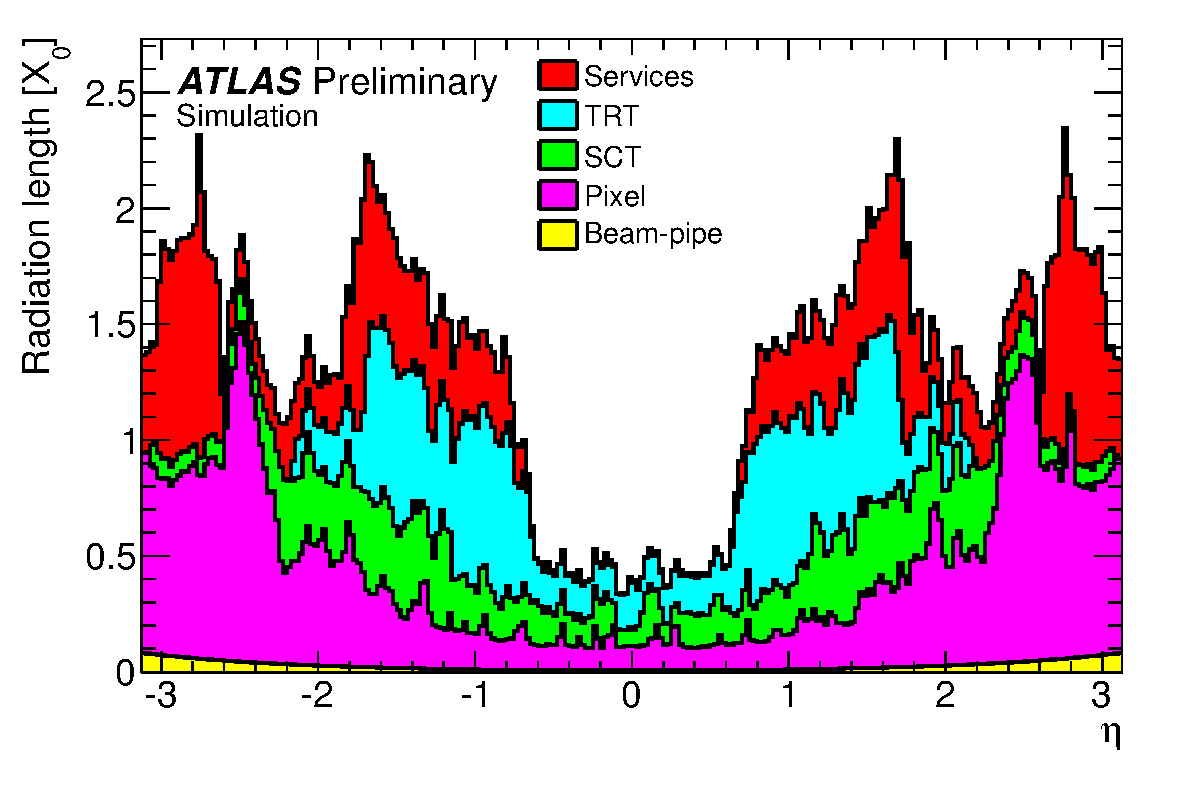
\includegraphics[width=0.8\textwidth]{id_material}
\caption[Distribution of the Inner Detector material for each sub-detector as a
function of the pseudorapidity.]{
Distribution of the Inner Detector material for each sub-detector as a
function of the pseudorapidity. The material of the Pixel and SCT detectors
includes passive material arising from electronics, cabling, cooling and
mechanical support. Figure from~\cite{ATLAS-CONF-2012-047}.}
\label{fig:id-material}
\end{figure}


The radiative loss of energy via \brem\ is highly non-Gaussian, and so is not
well modelled by the standard Kalman Filter, which can only incorporate Gaussian
noise terms. A non-linear extension of the
Kalman filter, the {\it Gaussian Sum Filter (GSF)}, has been
developed~\cite{Fruhwirth2003131,Atkinson:1448253}. It
approximates the PDF for energy loss from \brem\ as a weighted sum of Gaussian
components, and uses a separate Kalman Filter to process each one. For example,
one can consider the extrapolation of a measurement from a surface $k-1$ with state
described by $n_{k-1}$ components to surface $k$, where $\epsilon_{k}$ Gaussians
are used to describe the energy losses due to \brem\ between surfaces $k-1$ and
$k$. A separate Kalman Filter is then applied to each of the $n_{k-1}$
components, for each of the $\epsilon_{k}$ noise terms, resulting in the state at
surface $k$ being described by $n_{k} = n_{k-1} \cdot \epsilon_{k}$ components.
At each layer the number of components is artificially reduced to a fixed number
by merging similar components,
in order to make the extrapolation computationally feasible.
Using the GSF allows for better pattern recognition by picking up hits
occurring after kinks in tracks caused by \brem, as well as improving the
resolution of the track parameters.

%\subsubsection{2011 Improvements}

For 2011 data taking, `brem-refitting' was applied to
reconstructed electron candidates~\cite{ATLAS-CONF-2012-047}. For technical reasons, it was not possible to
include the \brem\ recovery from the beginning of electron reconstruction.
Instead, electrons were reconstructed using the standard pion hypothesis
tracking and track cluster matching as described above. The tracks of these candidates were then refitted
using the GSF algorithm. All tracks with \ptgtMeV{400} and \modetalt{2.5} assigned to
electron candidates were refitted, the cluster-track matching re-run
using the collection of refitted tracks, and the rest of the electron reconstruction
chain re-run using these refitted candidates. This led to the best matches between
cluster and track changing in approximately 5\% of cases at high pseudo-rapidity (0.8 \%
overall). However, since it was only possible to run the refitting on tracks
already associated to electron clusters using the standard tracking, the full
benefit of using GSF was not gained as many tracks with significant energy loss
from \brem\ would not be reconstructed successfully by the standard tracking and
thus could not be re-fitted. For this reason the brem-refitting did not
significantly improve the reconstruction efficiency, but did significantly
improve the resolution of track parameters in the bending plane such as \dzero, \dzerosig,
$\phi$ and \qoverp. For example, \fig{d0Sig-gsf} shows the impact parameter
significance (\dzerosig) distribution with and without the GSF refit. 

\begin{figure}[h!]
\centering
            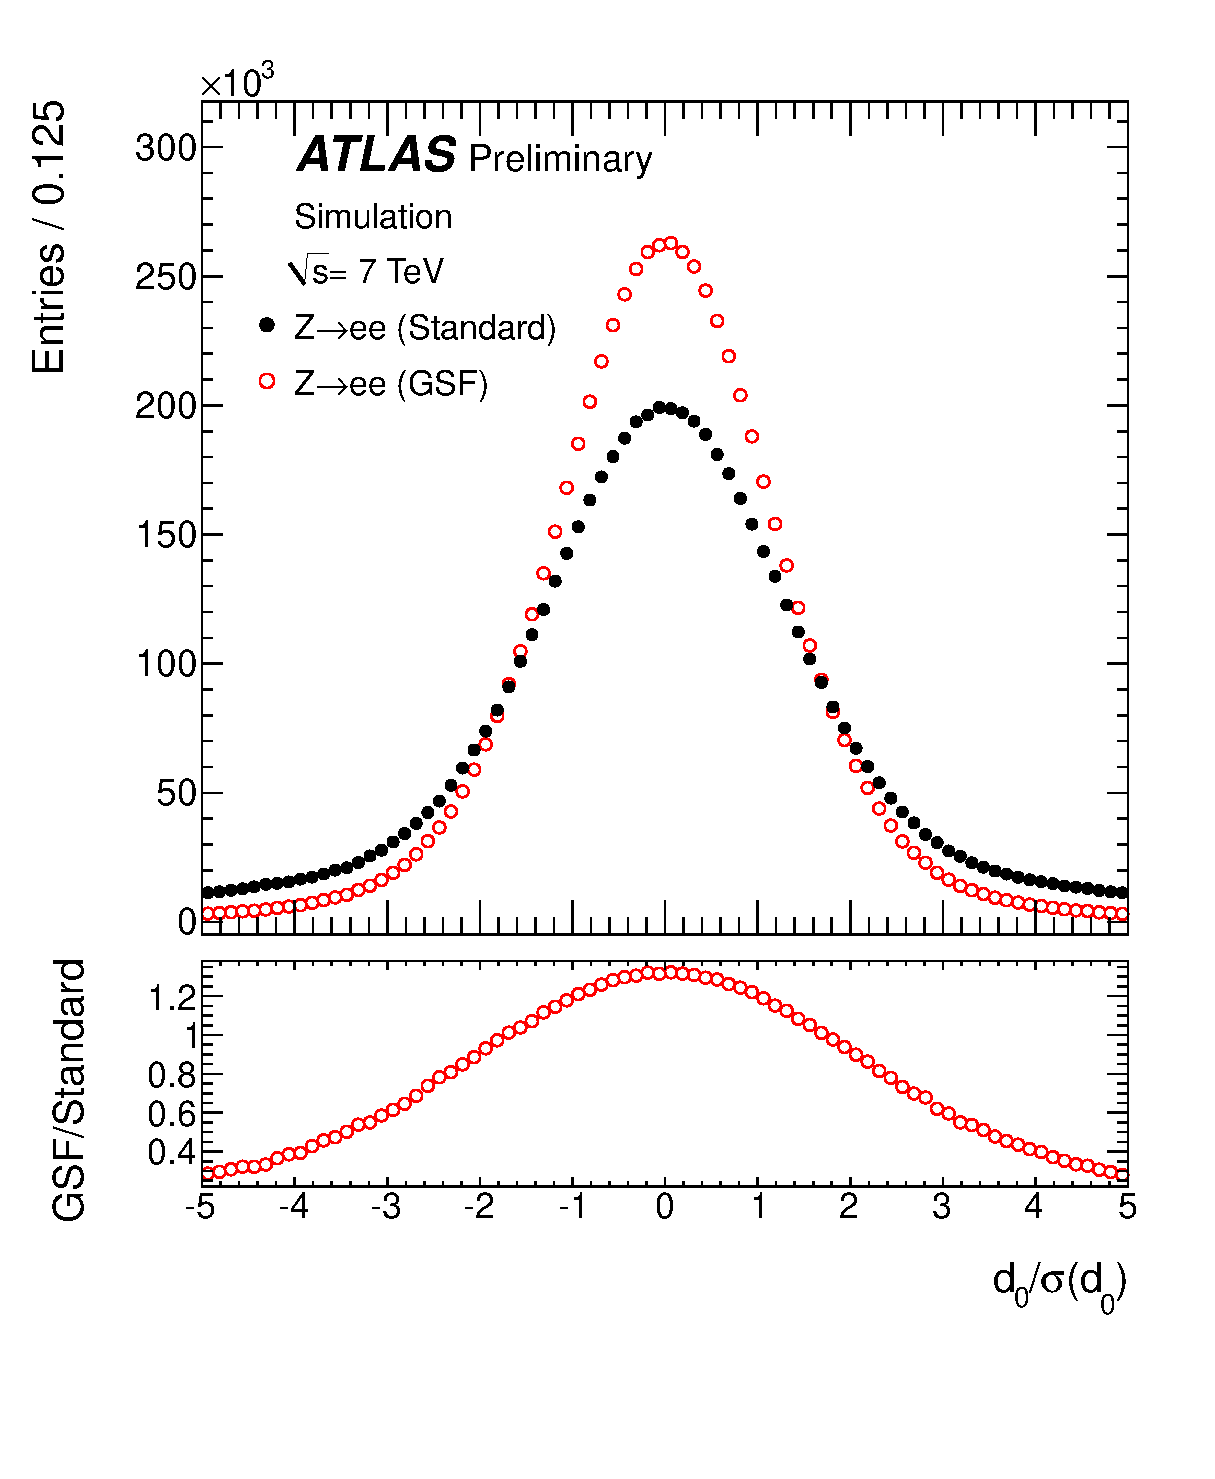
\includegraphics[width=0.7\textwidth]{d0Sig_gsf}
\caption[Distribution of the simulated transverse impact parameter significance for GSF (open
red) and standard (solid black) electrons from \Z-boson decays. ]{Distribution of the simulated transverse impact parameter significance for GSF (open
red) and standard (solid black) electrons from \Z-boson decays. 
%The bottom plots show the ratio of the entries of the GSF and standard
%electrons per bin
Figure from~\cite{ATLAS-CONF-2012-047}.}
\label{fig:d0Sig-gsf}
\end{figure}

%\subsubsection{2012 Improvements}

In 2012, improvements were made to all stages of the electron reconstruction
chain, from the initial tracking pattern recognition through to the track
cluster matching~\cite{HSG2:1456228}. 

Since the GSF tracking takes approximately 10 times more time to
run than the standard Kalman filter, it is not feasible to fit all tracks using
the GSF when doing the initial pattern recognition and track finding (see~\sec{tracking-std}). 
Additionally, the use of such a filter with electron hypothesis would
negatively affect non-electron tracks. Instead, the effects of \brem\ on
electron tracks are crudely modelled at the initial pattern recognition by allowing for 30\% energy loss at each surface for tracks with
momentum above 1 \gev. In order to avoid degrading non-electron tracks, this allowance is only made in regions of interest in a
cone of \deltaRlt{0.3} around EM calorimeter clusters. 

The global \chisquared\
fitter was also improved to allow for electron hypothesis tracks. Tracks
rejected due to low \chisquared\ at the ambiguity resolution stage in a RoI are
refitted using a modified `electron hypothesis' global \chisquared\ fitter. This
attempts to find the layer with the most significant \brem\ energy loss, then
reruns the fit with only an energy loss term for the most significant \brem\
loss. The advantage of this over the standard \chisquared\ fit, which allows
includes an energy loss term for each layer, is that in the latter approach the
electron momentum tends to be overestimated as all of the energy loss terms tend
to take the average energy loss value, rather than correctly identifying one layer with large
energy loss. The modified \chisquared\ fitter gives a significant improvement in the track
parameter resolution, giving an improvement almost as great as using the more
sophisticated GSF algorithm, but running in approximately one tenth of the time.

At this stage, there will still be a number of tracks which had large energy
losses from \brem\ and were consequentially badly fitted. A refit using the GSF
fitter described above is thus carried out for all tracks loosely matched to an
EM calorimeter cluster. Two forms are matching are carried out: the first
(\deltaR) between the
track parameters extrapolated to the second layer of the calorimeter and the
barycentre of the calorimeter cluster, and the second (\deltaR$^{\rm{rescaled}}$) where the track momentum is
scaled to the cluster energy before extrapolating the track to the calorimeter.
Loose cuts are made on \deltaR\ and \deltaR$^{\rm{rescaled}}$, with the cuts on
\deltaR$^{\rm{rescaled}}$ being slightly tighter.
Tracks which match under either of the two scenarios are refitted; the latter
category aims to select tracks with low momentum that have suffered large
\brem\ and would otherwise be missed. The final matching of the refitted tracks
to the clusters and selection of the best match is also improved; again both the
original \deltaR\ and the \deltaR$^{\rm{rescaled}}$ after scaling the track
momentum to the cluster
energy are computed. Tracks with Pixel detector hits are preferred. If there are
more than two tracks with Pixel hits matching to a cluster then the one with the smaller
\deltaR$^{\rm{rescaled}}$ is preferred, providing they are well enough
separated in \deltaR$^{\rm{rescaled}}$, otherwise the one with smaller \deltaR\
is chosen.

Overall these improvements increase the electron reconstruction efficiency by
$\sim2\%$ in the calorimeter barrel and $\sim5\%$ in the calorimeter endcaps.
For low \et\ electrons (\etlt{20}) the improvement is up to 6\%.

\subsubsection{Electron Reconstruction Efficiencies}

~\fig{el-reco-eff} shows the electron reconstruction efficiency in 2011 and 2012
as a function of the pseudo-rapidity and the transverse energy of the electron cluster.
The reconstruction efficiency in 2011 drops by approximately 4\% between central
and forward pseudo-rapidity. In 2012 the overall reconstruction efficiency
improves by approximately 2\% at central pseudo-rapidity, and the drop-off in
efficiency at high pseudo-rapidity is reduced to roughly 1\%. Similarly, the
reconstruction efficiency at low \et\ improves by roughly 6\% in 2012 with
respect to 2011. Good agreement is observed between the reconstruction
efficiency observed in data and the efficiency predicted by simulation.
Scale-Factors, parameterised as a function of $\eta$ and \et, are applied to
the Monte-Carlo to correct the reconstruction efficiency to that observed in
data.

\begin{figure}[h]
\centering
	\subfigure[]{
            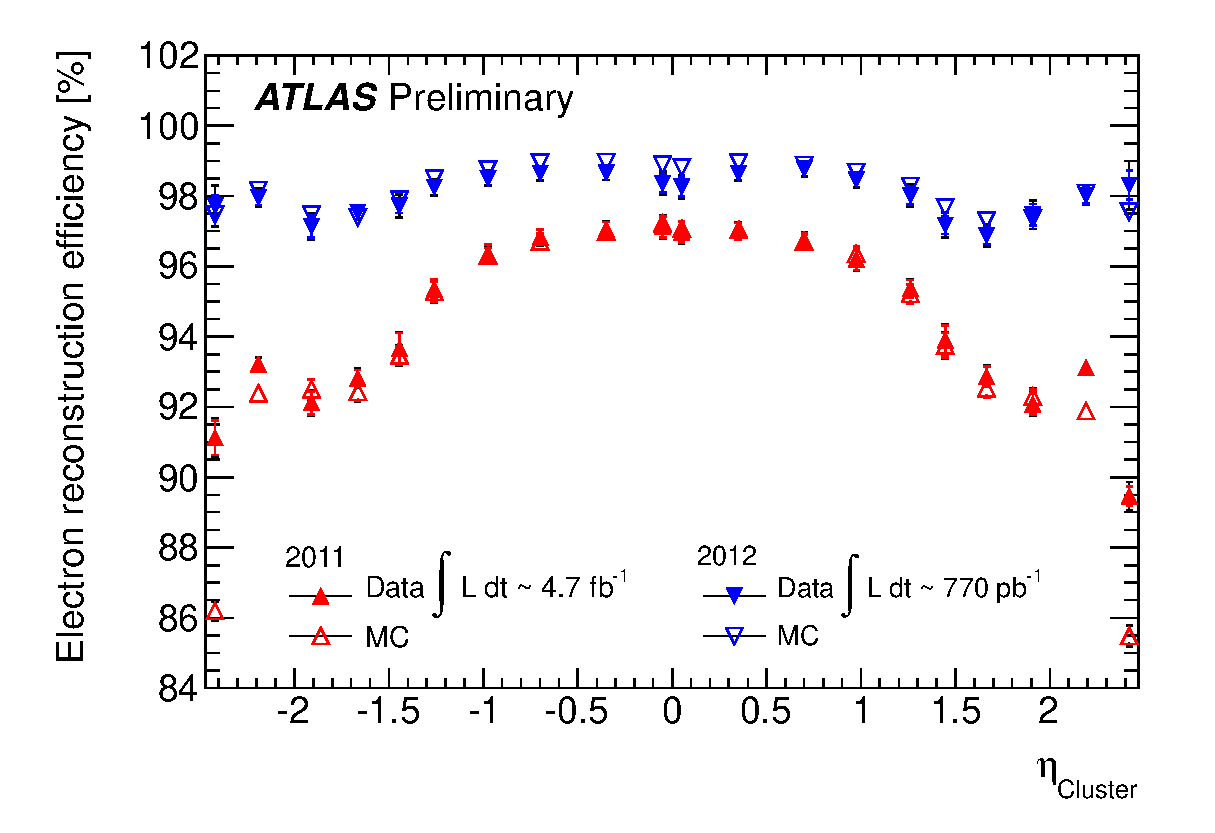
\includegraphics[width=0.47\textwidth]{ElRecoEffEtaBin2011_2012}
        }
	\subfigure[]{
            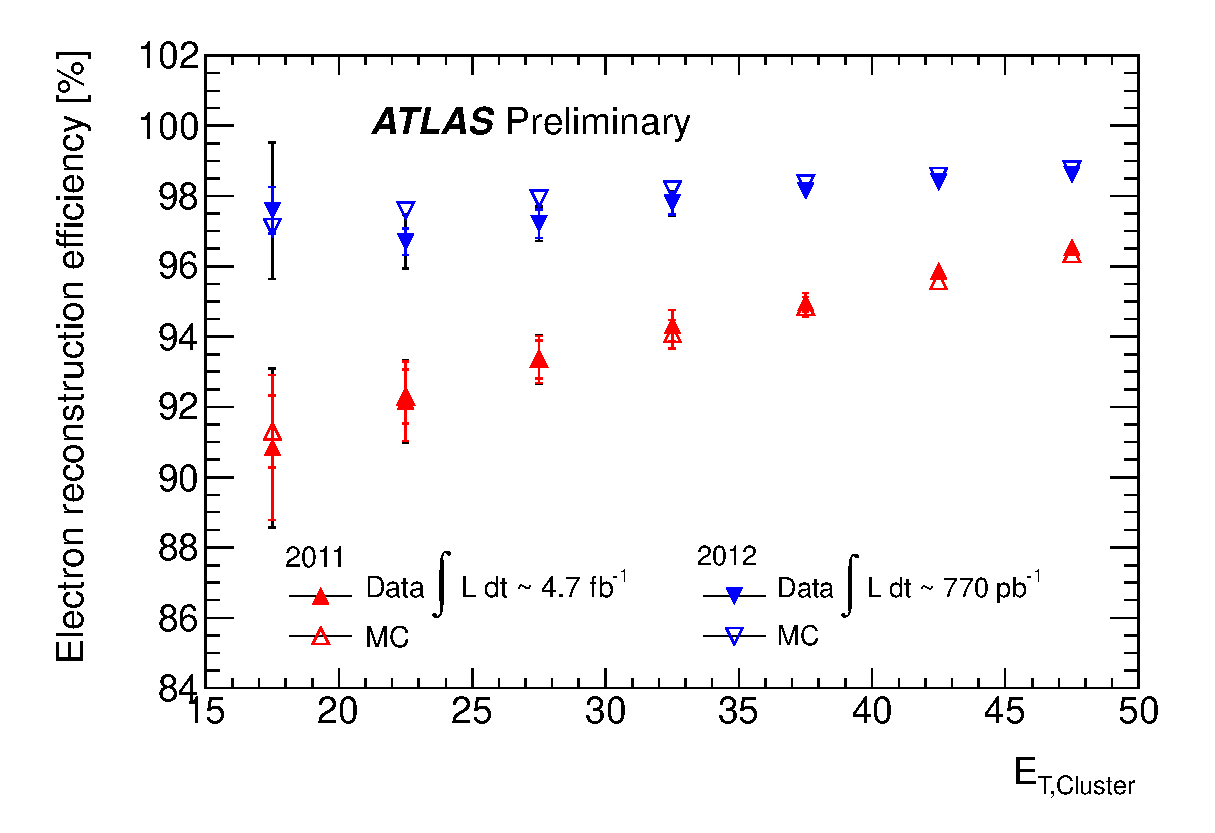
\includegraphics[width=0.47\textwidth]{ElRecoEffPtBin2011_2012}
        }
\caption[Electron reconstruction efficiency in 2011 and 2012 as a function of (a) the cluster
$\eta$ and (b) the cluster \et. ]{Electron reconstruction efficiency in 2011 and 2012 as a function of (a) the cluster
$\eta$ and (b) the cluster \et. The solid coloured points show the efficiency
observed in data whilst the open points show the simulated efficiency in
Monte-Carlo. Figures from~\cite{ElectronEfficiency2012}.}
\label{fig:el-reco-eff}
\end{figure}

\subsubsection{Electron Energy Calibrations}

A first measurement of the EM calorimeter energy scale is derived from test beam
measurements, however there are large uncertainties in the transfer
of the measurement from the test-beam to the actual ATLAS environment. Further,
the calorimeter energy response needs to be calibrated to account for the
varying amount of dead material before the calorimeters as a function of
pseudo-rapidity. \mc\ derived calibrations are applied
to the clusters to correct for dead material and leakage outside of the
calorimeter. The energy response is further calibrated in-situ using \Zee\
decays. This also allows the inter-calibration of different regions of the
calorimeters in $\eta$. The measured energy of an electron in region $i$ candidate can be
related to its true energy by:

\begin{equation}
E^{\rm meas} = E^{\rm true}(1 + \alpha_{i})
\end{equation}

where $E^{\rm true}$ is the true electron energy, $E^{\rm meas}$ is the measured
energy after applying the \mc\ based energy-scale correction and $\alpha_{i}$
measures the residual mis-calibration. The residual calibrations are determined
by selecting pairs of opposite-sign high \pt\ electrons with a di-electron
invariant mass near to the \Z\ peak. The $\alpha$ parameters are obtained by
performing an unbinned fit minimising the log-likelihood function:

\begin{equation}
-\ln L_{\rm tot} = \sum_{i,j} \sum^{N^{\rm events}_{ij}}_{k} -\ln
L_{ij} \left( \frac{m_{k}}{1+\frac{\alpha_{i} + \alpha_{j}}{2}} \right)
\end{equation}

where $i,j$ label the $\eta$ regions of the two electrons from the \Zee\ decay,
$m_{k}$ is the measured di-electron mass (after applying the test-beam and \mc\
calibrations) in event $k$ and $L_{ij}(m)$ is a probability density function
describing the likelihood of observing a \Zee\ decay with mass $m$. The pdf is
taken from \mcsim. The resulting calibration parameters $\alpha_{i}$, measured
in 2010 data, are shown in~\fig{el-energy-calib-const-2010}.
Figures~\ref{fig:el-energy-calib-time-2011}
and~\ref{fig:el-energy-calib-time-2012} show the calibration parameters measured
as a function of time in 2011 and 2012 respectively, and
Figures~\ref{fig:el-energy-calib-pu-2011}
and~\ref{fig:el-energy-calib-pu-2012} show the parameters as a function of
the average number of interactions per bunch crossing due to pileup for 2011 and 2012 data respectively. The calibration is found
to be constant in time, and insensitive to pileup. The linearity of the response
with respect to electron energy is checked by applying a similar procedure to electrons
from \JPsiee\ decays (for which the sample is much more statistically limited).
The results are found to be in good agreement with the results from \Zee\
decays, and the resulting difference is assigned as an energy scale systematic
at low \et.

\begin{figure}[h!]
\centering
	\subfigure[]{
            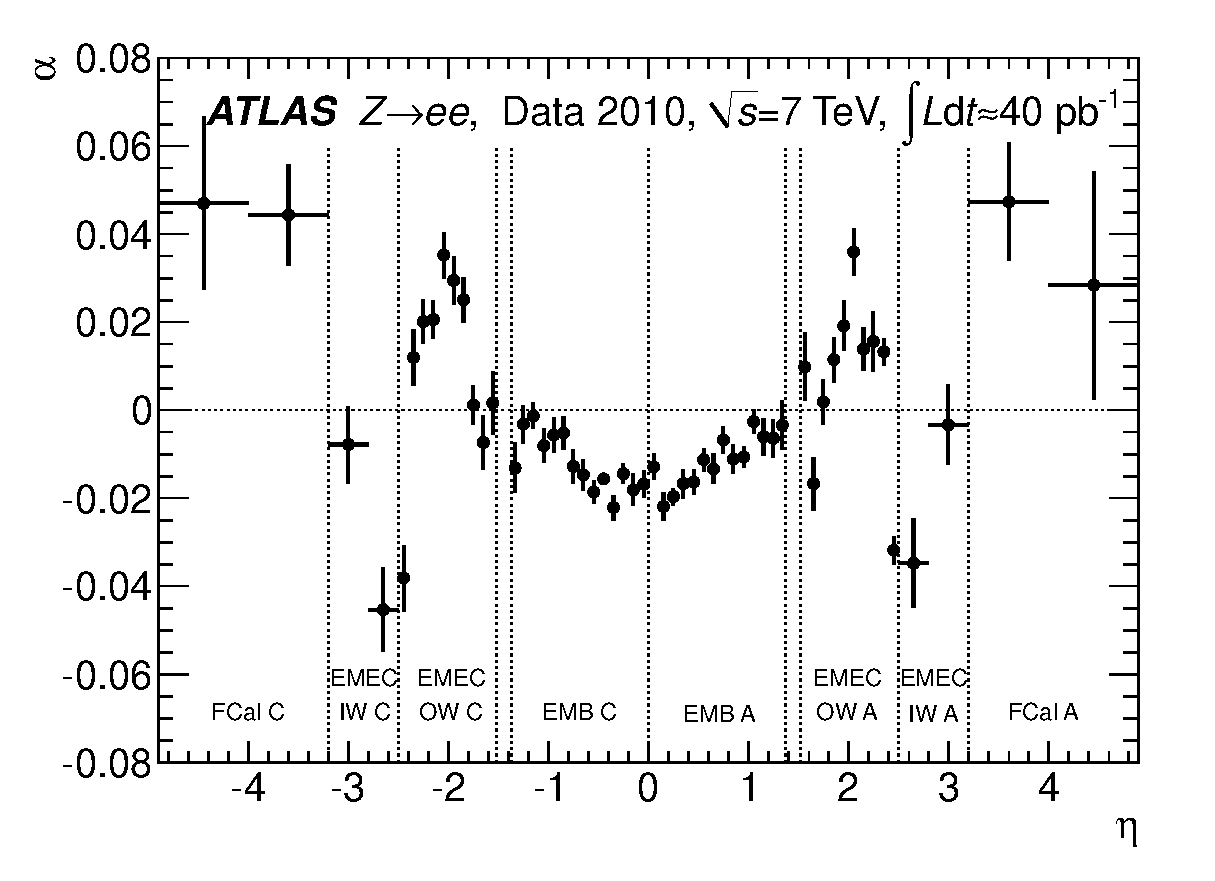
\includegraphics[width=0.47\textwidth]{el_energy_response_eta_2010}
\label{fig:el-energy-calib-const-2010}
        }
        \hspace{10mm}
	\subfigure[]{
            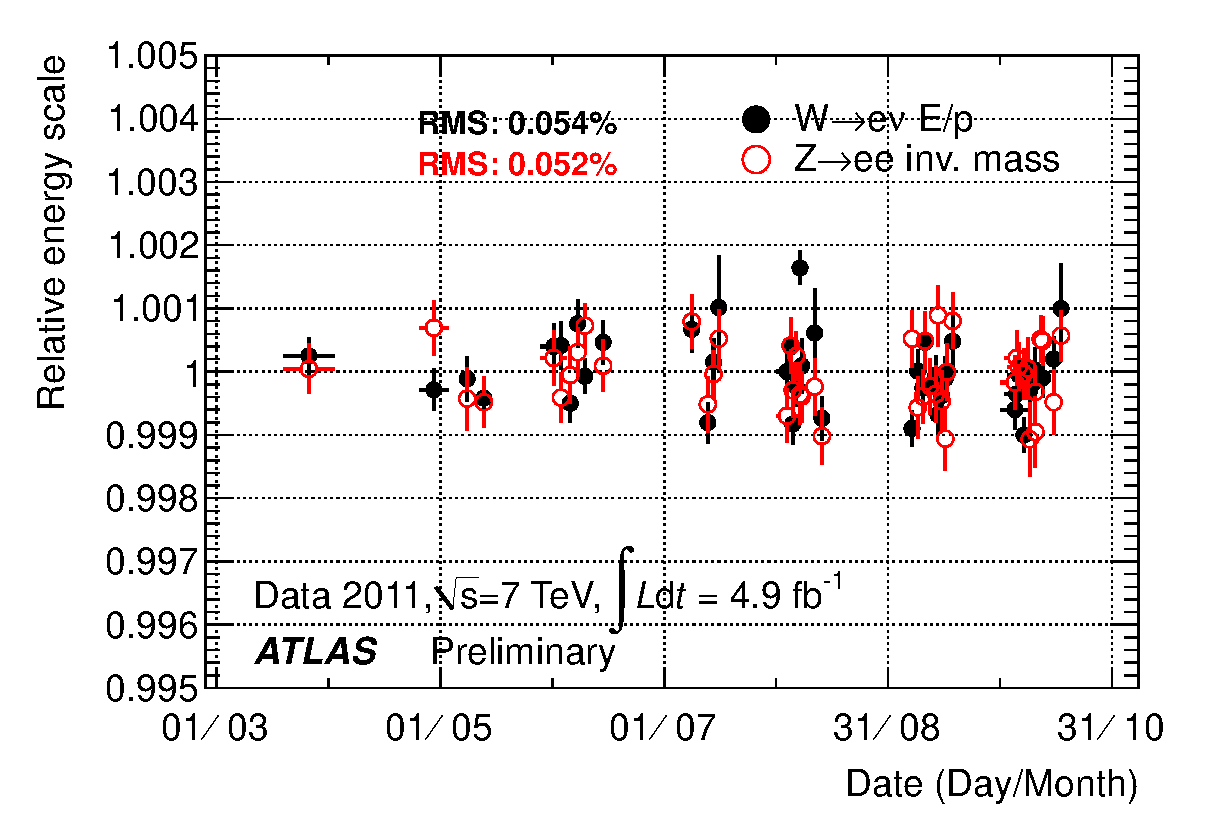
\includegraphics[width=0.47\textwidth]{el_energy_response_time_2011}
\label{fig:el-energy-calib-time-2011}
        }
	\subfigure[]{
            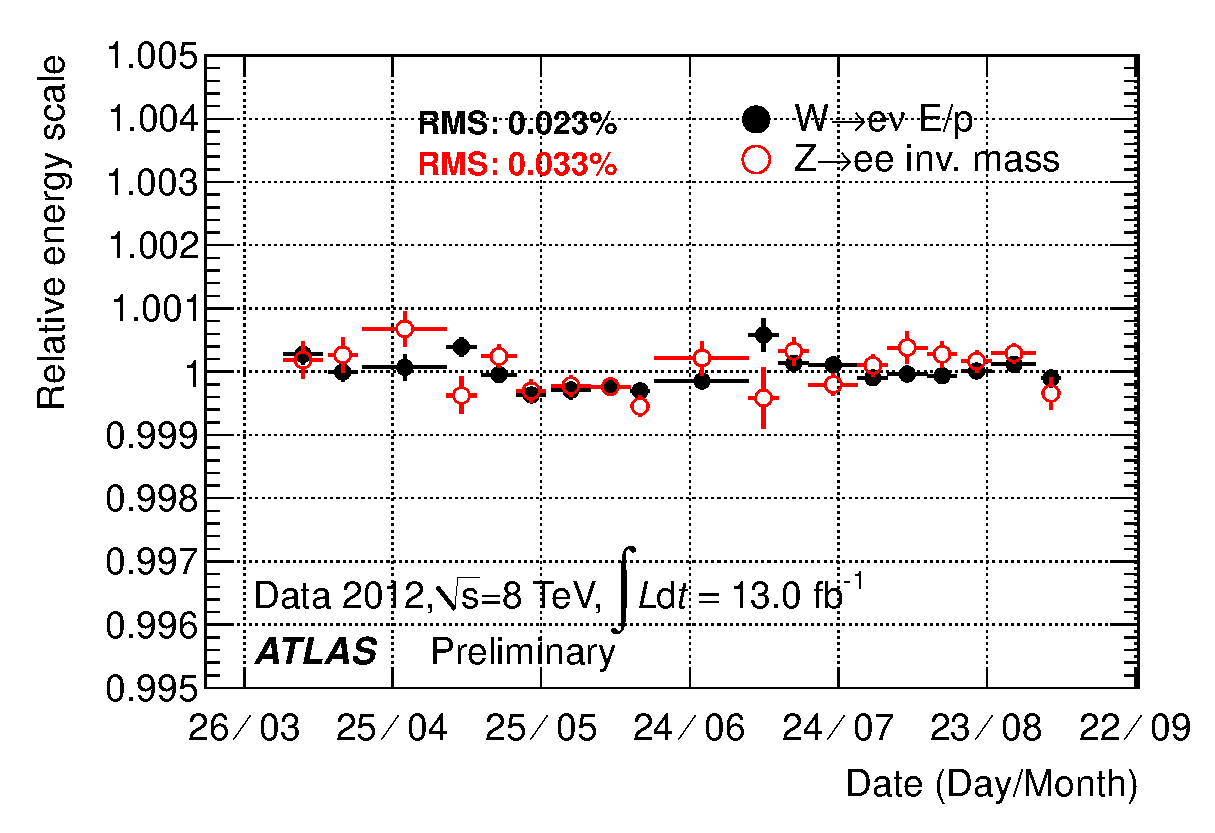
\includegraphics[width=0.47\textwidth]{el_energy_response_time_2012}
\label{fig:el-energy-calib-time-2012}
        }
	\subfigure[]{
            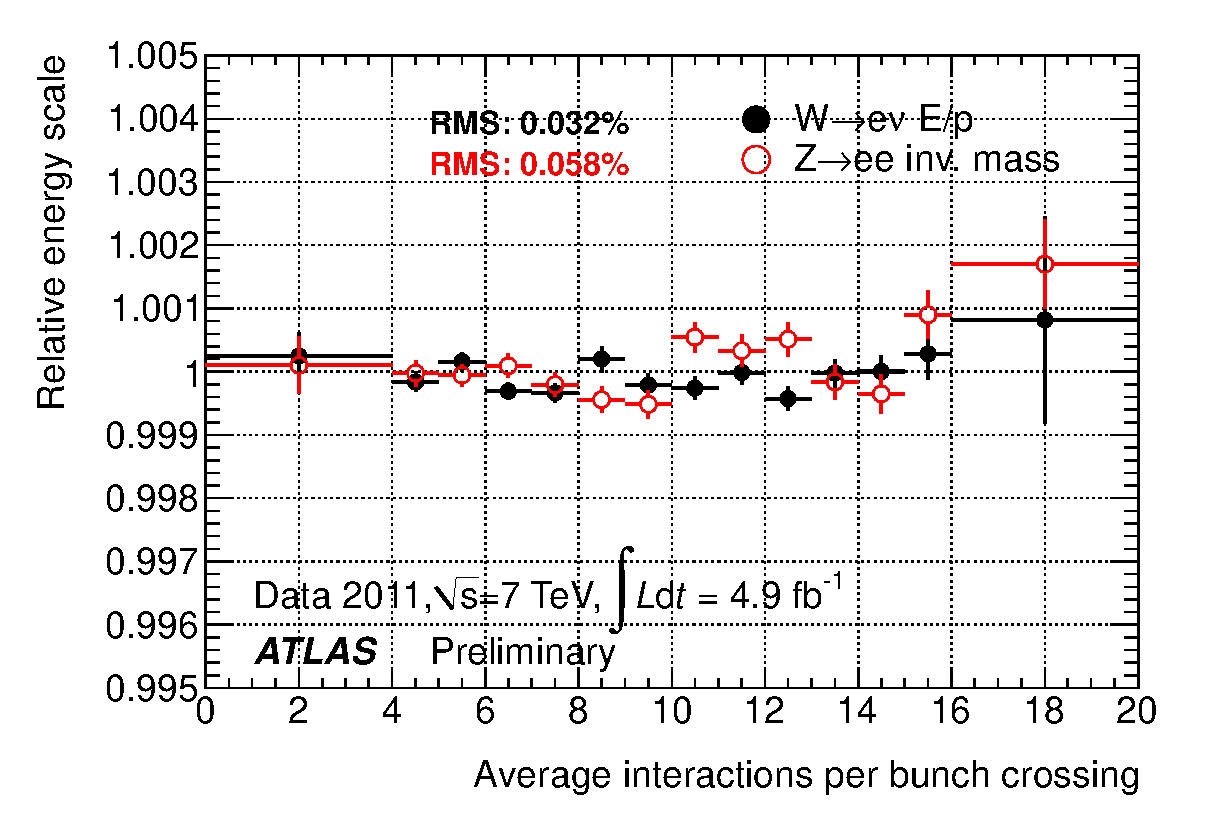
\includegraphics[width=0.47\textwidth]{el_energy_response_pu_2011}
\label{fig:el-energy-calib-pu-2011}
        }
	\subfigure[]{
            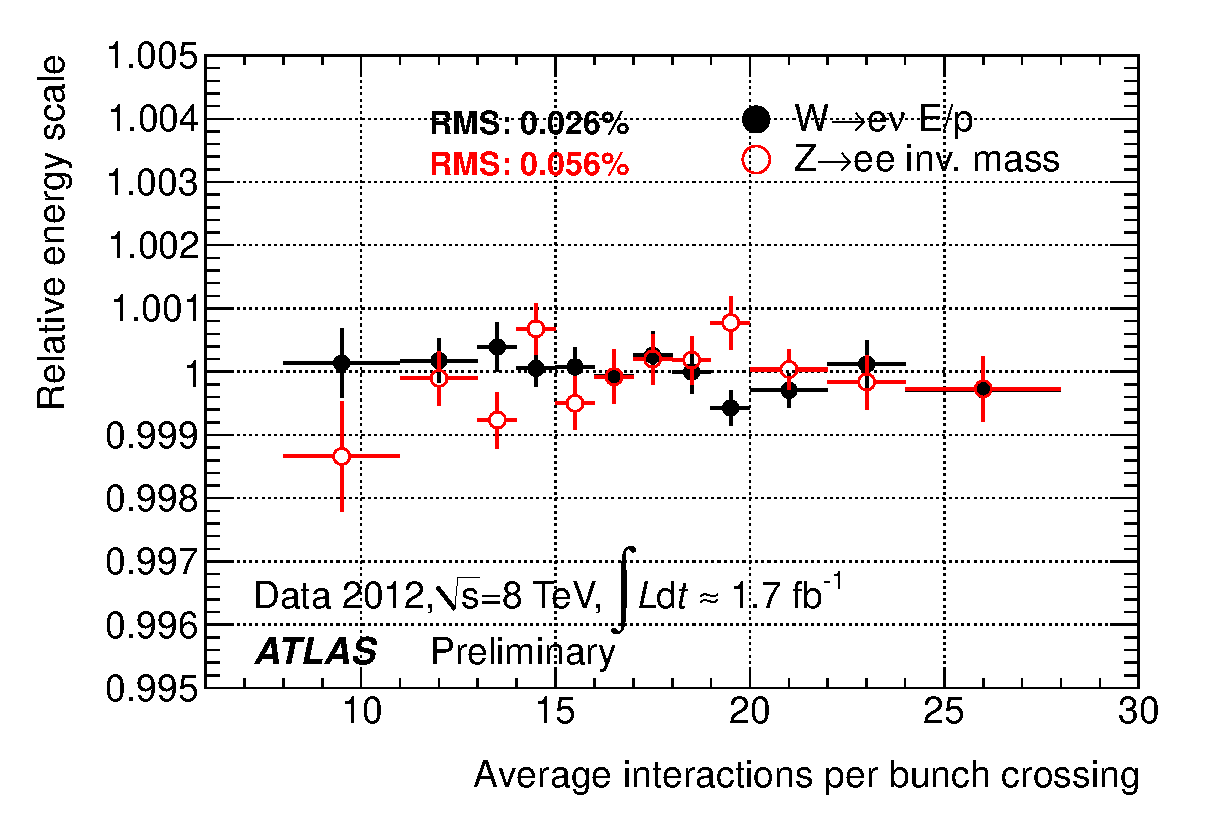
\includegraphics[width=0.47\textwidth]{el_energy_response_pu_2012}
\label{fig:el-energy-calib-pu-2012}
        }
\caption[Electron energy-scale correction factor $\alpha$ derived from fits to
\Zee.]{
Figure (a) shows the energy-scale correction factor $\alpha$ as a function of the
pseudorapidity of the electron cluster derived from fits to \Zee\ in
2010~\cite{Aad:2011mk}. The errors shown are statistical only.
Figures (b) and (c) show the stability of the energy-scale correction factor
$\alpha$ (integrated over all $\eta$) in 2011~\cite{ElectronEnergyTimePileup2011} and 2012~\cite{ElectronEnergyTime2012} respectively. Figures (d)
and (e) show the stability with respect to pile-up in 2011~\cite{ElectronEnergyTimePileup2011} and
2012~\cite{ElectronEnergyPileup2012}
respectively.}
\label{fig:el-energy-calib-const}
\end{figure}

The electron energy resolution is also measured in data. ~\fig{el-energy-calib-2011} shows the observed di-electron 
mass distribution for all $\eta$ bins for data taken in 2011 after applying the
energy calibration described above. The distribution
is fit to a Breit-Wigner to model the \Z\ lineshape convolved with a
Crystal-Ball function to model the detector resolution and effects of FSR. The
parameters of the Breit-Wigner are fixed to those of the \Z\ boson. The
resolution observed in data is slightly worse than the simulated resolution; a
Gaussian smearing is applied to electron energies in the simulation to reproduce the resolution observed in the data.

\begin{figure}[h]
\centering
            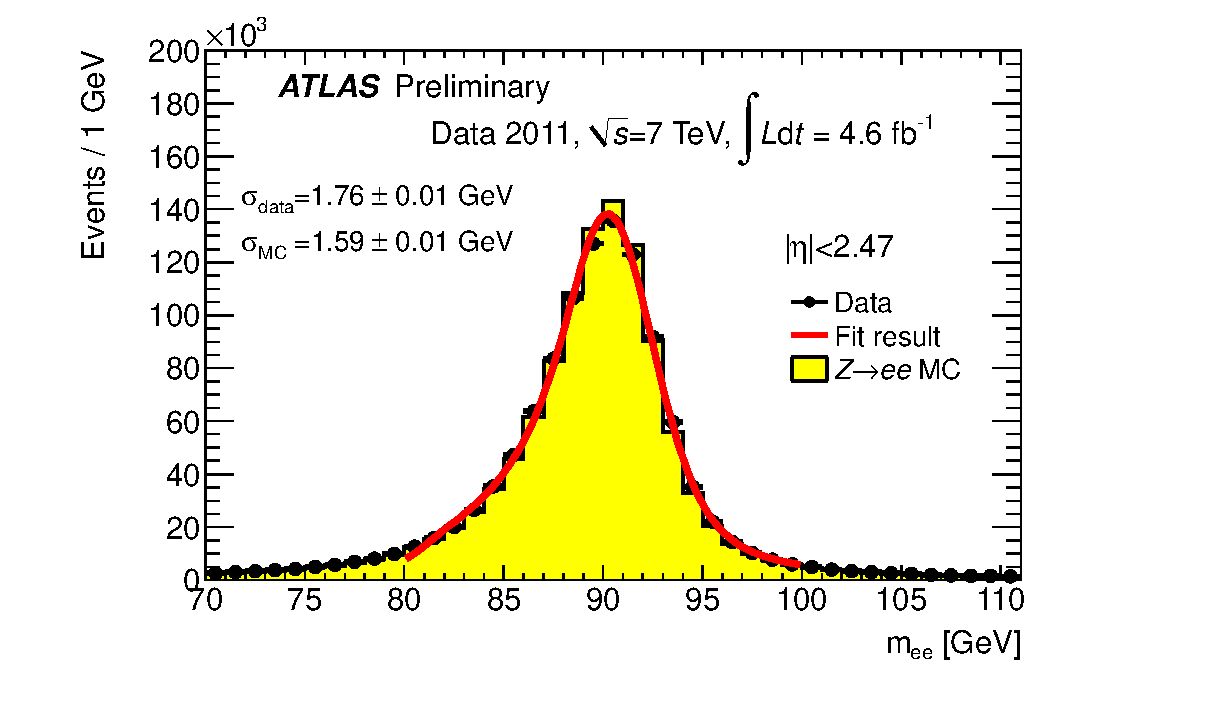
\includegraphics[width=0.8\textwidth]{zee_mass_calibration_2011}
\caption[Di-electron mass distribution after applying the
energy scale calibration. ]{Di-electron mass distribution after applying the
energy scale calibration. The points show the distribution observed in data
whilst the histogram shows the prediction from simulation. The red line shows a
fit to the data 
using a Breit-Wigner convolved with a
Crystal-Ball function in order to determine the resolution. Figure from~\cite{ElectronZee2011}.}
\label{fig:el-energy-calib-2011}
\end{figure}

\subsection{Electron Identification}
\label{sec:reco-el-id}

The electron candidates reconstructed as described in the previous section will
contain a high contamination from jets faking electrons, non-isolated electrons
from decays in jets and electrons from photon conversions. In order to identify
prompt isolated electrons a
cut based identification is used. Cuts are made on variables relating to the
shape of the electromagnetic shower in the calorimeter, the quality of the Inner Detector track, the
track-calorimeter matching and particle identification information from the
TRT. The cuts were optimised using a multivariate analysis program (TMVA), in 10 bins
of cluster $\eta$ and 11 bins of cluster \et\ from 5 \gev\ to $>80$ \gev.
Three reference sets of cuts are used, denoted \loose, \medium\ and \tight,
designed to give progressively greater background rejection, at the cost of
signal efficiency. The expected jet rejections (from simulation) of the three points are 500, 5000
and 50000 respectively~\cite{ATL-PHYS-PUB-2011-006}.

In order to maintain manageable trigger rates with increased instantaneous
luminosity, the original \loose, \medium\ and \tight\ were re-optimised in order
to increase background rejection. The new working points are denoted \loosePP,
\mediumPP\ and \tightPP. In 2012, the identification was further re-optimised to
prevent drops in efficiency in events with high pileup of up to 20\%. 

\subsubsection{\loosePP\ Requirements}

In both 2011 and 2012 \loosePP\ cuts on shower shape variables in the first and
second layers of the EM calorimeter, leakage into the hadronic
calorimeter, track quality in the silicon detectors and loose track cluster
matching. The variables cut on are as follows:

\begin{itemize}

    \item {\bf Shower Shapes:} cuts are made on the following shower shape
    variables:

    \begin{itemize}
        \item Hadronic leakage, \Rhad, the ratio of \et\ in the first layer of
        the hadronic calorimeter to the \et\ of the EM cluster. In the range
        \modetabetween{0.8}{1.37} the \et\ of the full hadronic calorimeter is
        used, to compensate for the crack between the barrel and extended barrel
        of the tile calorimeter.
        \item The ratio of the energy in the middle layer of the
        calorimeter in $3 \time 7$ cells to the energy in $7
        \times 7$ cells centered at the electron cluster position, \Reta.
        \item Lateral width of the shower in the second layer of the EM
        calorimeter, \wetatwo.
        \item Ratio of the energy difference between with the largest and second
        largest energy deposit in the first layer of the EM calorimeter over the
        sum of their energies, \Eratio.
        \item Total width of the shower in the first layer of the EM
        calorimeter, \wstot.
    \end{itemize}

    \item {\bf Silicon Hits:} at least 7 hits in the silicon detectors, of which at
    least one must be in the pixel detector. This ensures good track quality and
    rejects backgrounds from conversions or Dalitz-decays.
    \item {\bf Track-Cluster matching:} a loose matching in $\eta$ is applied,
    requiring \deltaetalt{0.015}
\end{itemize}

The shower shape variables \Reta\ and \Rhad\ are particularly susceptible to
pileup since they sample a large area of the calorimeter. Cuts on these
variables were therefore
loosened in 2011 with respect to 2012, reducing the rejection power of \loosePP\
by about 20\%.

\subsubsection{\mediumPP\ Requirements}

All \loosePP\ cuts are required to be passed, and in addition:

\begin{itemize}
    \item {\bf Shower Shapes:} the shower shape cuts made in \loosePP\ 
    (\Reta, \Rhad, \wetatwo, \Eratio, \wstot) are made at tighter values. For
    2012, the cuts on \Reta\ and \Rhad\ were loosened with respect to 2011, and
    made at the same value as for \loosePP, whilst the cuts on  \wetatwo, \Eratio\ and
    \wstot\ were tightened with respect to 2011.

    \item {\bf Track-Cluster matching:} a tighter matching in $\eta$ is applied,
    requiring \deltaetalt{0.005}.

    \item {\bf Impact Parameter:} require that the electron's track has a
    transverse impact parameter \dzero $<$ 5 mm.

    \item {\bf Silicon Hits:} stricter requirements are made on hits in the
    silicon detectors. It is requireq that there is at least one hit in the b-layer for
    \modetalt{2.01} (\modetalt{2.37} in 2012). In 2011, at least 1
    Pixel hit is required for \modetalt{2.01} and at least two for
    \modetagt{2.01}. For 2012, two Pixel hits are required in all bins.

    \item {\bf Fraction in third calorimeter layer \fthree:} for 2012 a cut on the
    fraction of the shower energy deposited in the third layer of the EM
    calorimeter was added to compensate for the loosening of the cuts in the
    first layer of the calorimeter. This cut is only applied for \etlt{80}, since
    the depth of the EM shower and hence leakage into the third layer increases
    with energy.

    \item {\bf TRT High Threshold Hits} A loose requirement is made on the
    fraction of high-threshold (HT) hits from transition radiation photons in the
    TRT detector (see~\sec{Detector-TRT}).

\end{itemize}

\subsubsection{\tightPP\ Requirements}


All \mediumPP\ cuts are required to be passed, and in addition:

\begin{itemize}
    \item {\bf Shower Shapes:} cuts on shower shape variables are made at equal
    or tighter values to those for \mediumPP. As for \mediumPP,
    the cuts on \Reta\ and \Rhad\ were loosened in 2012 with respect to 2011, 
    whilst the cuts on  \wetatwo, \Eratio\ and
    \wstot\ were tightened.

    \item {\bf Track-Cluster matching:} a cluster matching in $\phi$ is added,
    requiring \deltaphilt{0.02}, and cuts are made on the ratio of the cluster
    energy to the track momentum, \Eoverp.

    \item {\bf Impact Parameter:} the
    transverse impact parameter cut is tightened to \dzero\ $<$ 1 mm.

    \item {\bf Silicon Hits:} stricter requirements are made on hits in the
    silicon detectors, requiring that there is at least one hit in the b-layer for
    all $\eta$, and, in 2012, at least 2 hits in the Pixel detector for all
    $\eta$.

    \item {\bf Conversion Rejection:} candidates matched to reconstructed photon
    conversions are rejected.

\end{itemize}

\subsubsection{Forward Electron Identification}

Since in the forward region there is no tracking from the Inner Detector,
identification in the forward region must rely on calorimeter shower shape
variables alone. A good discrimination between electrons and hadrons may be made
due to the fine transverse and longitudinal segmentation of the calorimeter, but
it is not possible to distinguish electrons and photons in the forward regions.
Two reference sets of cuts are defined for forward electrons, \loose\ and
\tight.

\subsubsection{Forward \loose\ Requirements}

Cuts are made on the following variables:

\begin{itemize}
    \item {\bf Shower depth, $\lambda_{\rm centre}$} the distance of the shower
    barycentre from the front face of the calorimeter along its axis.  
    \item {\bf Longitudinal Second Moment, $\langle \lambda^2 \rangle$} the second
    moment\footnote{The $n^{\rm th}$ moment is defined as $\langle x^n \rangle =
    \frac{\sum_{i} E_i x^n_i}{\sum_{i} E_i}$ where $i$ runs over all cells in the
    cluster.} of the distance of each cell to
    the shower barycentre in the longitudinal direction.  
    \item {\bf Transverse Second Moment, $\langle r^2 \rangle$} the second moment of the 
    distance of each cell to the shower barycentre in the transverse direction.
\end{itemize}

\subsubsection{Forward \tight\ Requirements}

All of the \loose\ cuts are required to be passed, an in addition cuts are made
on the following variables:

\begin{itemize}
    \item {\bf Fraction Fraction of cluster energy in the most energetic cell,
    $f_{\rm max}$.}
    \item {\bf Normalized lateral moment, $\frac{w_{2}}{w_{2} + w_{\rm max}}$} where
    $w_{2}$ is the second moment of $r_{i}$ setting $r_{i} = 0$ for the two most
    energetic cells and $w_{\rm max}$ is the second moment of $r_{i}$ setting
    $r_{i} = 4$ cm for the two most energetic cells and $r_{i} = 0$ for the
    remaining cells.
    \item {\bf Normalized longitudinal moment, $\frac{l_{2}}{l_{2} + l_{\rm
    max}}$}
    where, similarly to the normalised longitudinal moment, 
    $l_{2}$ is the second moment of $\lambda_{i}$ setting $\lambda_{i} = 0$ for the two most
    energetic cells and $l_{\rm max}$ is the second moment of $\lambda_{i}$ setting
    $\lambda_{i} = 10$ cm for the two most energetic cells and $\lambda_{i} = 0$ for the
    remaining cells.
\end{itemize}

\subsubsection{Electron Identification Efficiencies}

\begin{figure}[h]
\centering
	%\subfigure[]{
            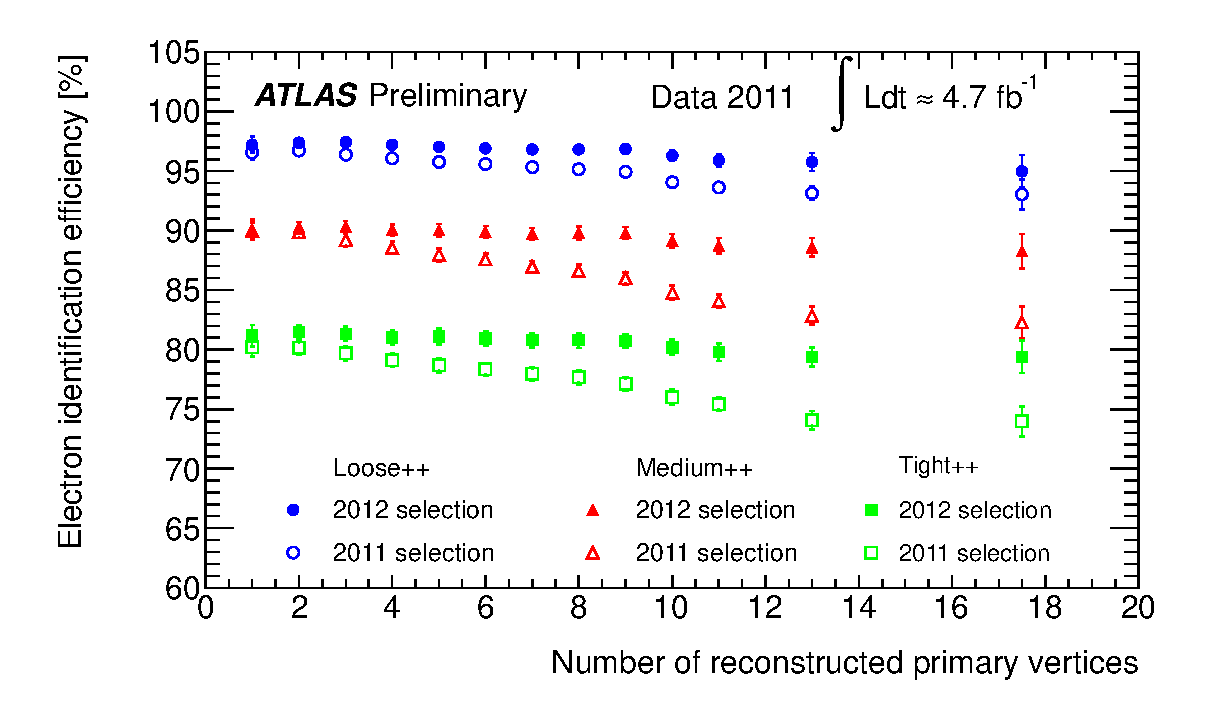
\includegraphics[width=0.8\textwidth]{data_effPP_vs_pvx_2011_2012}
        %}
	%\subfigure[]{
            %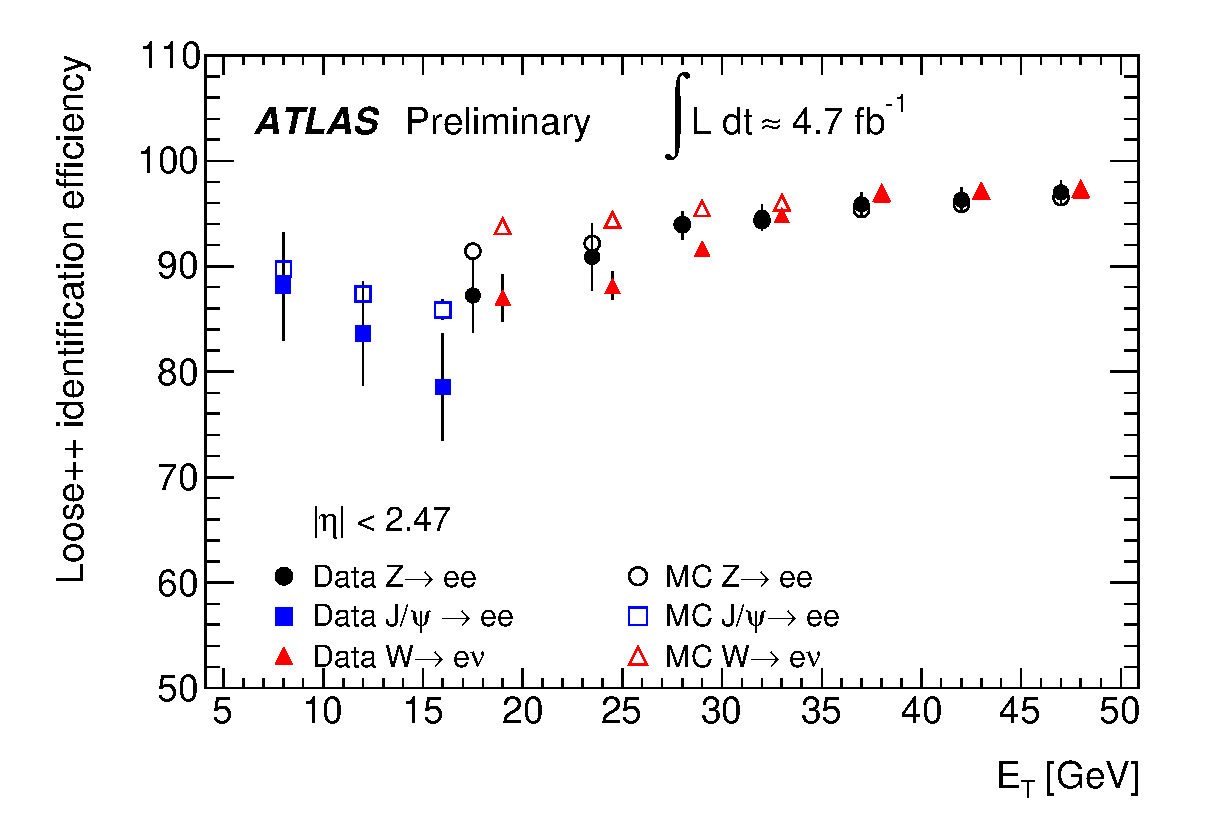
\includegraphics[width=0.7\textwidth]{ElLoosePPEfficiencyPt2011}
        %}
\caption[Electron identification efficiency in 2011 and 2012
 as a function of the number of reconstructed primary vertices in
the event. ]{Electron identification efficiency in 2011 (open markers) and 2012
(solid markers) as a function of the number of reconstructed primary vertices in
the event. The blue circles show the efficiency for the \loosePP\ selection, the
red triangles for the \mediumPP\ and the green squares for the \tightPP. 
Figure
from
~\cite{EfficiencyPileup}.
%~\cite{ElectronEfficiency2012,EfficiencyPileup,ElectronEfficiency2011,ElectronEffPV2011}.
}
\label{fig:el-id-eff-npv}
\end{figure}

~\fig{el-id-eff-npv} shows the electron identification efficiency in 2011 and 2012
as a function of the number of reconstructed primary vertices in the event.
Using the 2011 identification requirements, the efficiency can drop by over 5\%
in events with 18 reconstructed primary vertices with respect to the efficiency
in events with a single primary vertex.
~\fig{el-id-eff-et} shows the \loosePP\ identification efficiency as a function
of \et, using the 2011 requirements. Differences at the level of a
few percent are observed between the efficiency measured in data and the
efficiency measured in Monte-Carlo simulation. This is mainly attributed to mis-modelling
of the shower shape variables in the Monte-Carlo.
Scale-Factors, parameterised as a function of $\eta$ and \et, are applied to
the Monte-Carlo to correct the reconstruction efficiency to that observed in
data.


\begin{figure}[h]
\centering
            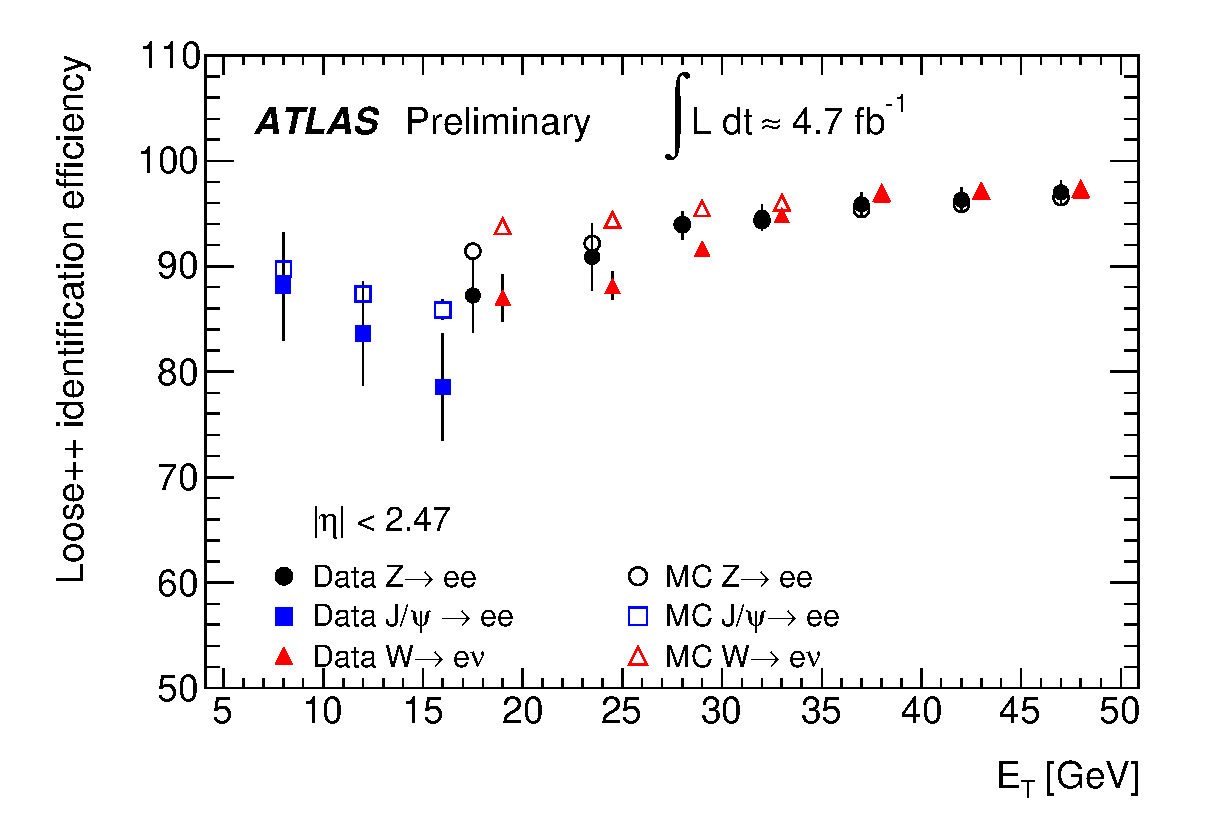
\includegraphics[width=0.8\textwidth]{ElLoosePPEfficiencyPt2011}
\caption[Efficiency of
the \loosePP\ identification requirements as a function of the cluster transverse
energy.]{
Efficiency of
the \loosePP\ identification requirements as a function of the cluster transverse
energy. The solid points indicate data based measurements whilst the open points
indicate predictions from Monte-Carlo. The different markers indicate the method used to
measure the efficiency: results from \Zee\ tag and probe are shown as black
circles, results from $\jpsi \ra ee$ as blue squares and results from $W \ra e
\nu$ as red triangles.
Figure
from
~\cite{ElectronEfficiency2011}.
%~\cite{ElectronEfficiency2012,EfficiencyPileup,ElectronEfficiency2011,ElectronEffPV2011}.
}
\label{fig:el-id-eff-et}
\end{figure}


%The cluster reconstruction efficiency is very efficient for electrons:


\section{Muon Reconstruction and Identification}
\label{sec:reco-mu}

\subsection{Muon triggers}
\label{sec:reco-mu-triggers}
